%!TEX root = ../main.tex

Le deuxième chapitre de ce mémoire parlera sur les différents techniques utilisés par les virus 
dans le processus d'infection, ainsi que les techniques employées par ces derniers pour dissimuler leurs présences.

Ce chapitre portera aussi sur différentes notions qui ont une relation plus ou moins indirecte avec les virus,
et qui sont nécessaires pour la réalisation d'une études plus propre et plus claire.

\newpage

% \section{Infection virale}
    % \subsection{Introduction}

\section{Classification des virus par cible}
L'un des moyens de classifications des virus est de voir ce qu'ils essayent d'infecter.
Dans cette section, trois classes de virus seront abordées : les virus visant les programmes, les virus système,
et les virus interprétés.

    \subsection{Virus visant programme}
    Les virus qui visent les programmes, cherchent à infecter les exécutables binaires compilés. 
    Le principe de fonctionnement est le suivant : le virus est présent dans un fichier exécutable, lorsque 
    ce dernier est exécuté, le virus choisit et contamine un ou plusieurs autres fichiers ; si le virus se maintient
    en mémoire, il infecte d'autres fichiers à l'exécution, ou simplement lors d'une manipulation. %vérifié

    Il existe plusieurs types de programmes, et chacun d'eux peut faire l'objet d'une attaque virale spécifique :
    \begin{description}
        \item[Programmes DOS :] Jusqu’en 1999, la majorité des virus programmes fonctionnaient sous 
            DOS et ciblaient les fichiers exécutables par ce système d'exploitation. 
            Déjà limitée à cette époque, la proportion des infections dues à ces virus DOS n’a cessé 
            de diminuer pour être presque inexistante aujourd’hui.
        \item[Application Windows 16 bits :] Ces programmes sont aussi appelés \emph{New Executable} (NE EXE).
            Ils sont rencontrés dans les environnements Windows 3.x. 
        \item[Application Windows 32 bits :] Ces programmes sont aussi appelés \emph{Portable Executable}
            (PE EXE). Ils sont rencontrés dans les environnement Windows actuel.
    \end{description}

    % Pour cette classe, les virus choisissent l'une des trois techniques, présentés ci-dessous, 
    % pour infecter les fichiers exécutables.
    %     \subsubsection{Ajout au début du fichier}
    %     Les anciens format exécutable traités tout le fichier comme une combinaison de code et de données.
    %     Quand le fichier est exécuté, ce dernier est chargé complètement en mémoire, et l'exécution commence
    %     du début du fichier.

    %     Avec ce type d'exécutable, si le virus s'ajoute au début du fichier, il obtiendra le contrôle 
    %     automatiquement dés l'exécution de ce dernier. Cette technique d'infection est relativement facile,
    %     mais ce n'est pas la méthode la plus simple d'infecter un fichier.

    %     \subsubsection{Ajout à la fin du fichier}
    %     Cette technique implique que le virus ajoute son code à la fin du fichier exécutable. C'est facile
    %     à mettre en place, et ça demande pas beaucoup d'effort.

    %     Comment le virus obtient-il le contrôle en utilisant cette méthode ? Il y a deux possibilités :
    %     \begin{itemize}
    %         \item Une ou plusieurs instructions du code original peuvent être sauvegardées, et remplacées 
    %             par une instruction de saut inconditionnel vers le code viral. 
    %             Plus tard, le virus remettra le contrôle au code qu'il a infecté. Le virus pourra 
    %     \end{itemize}

    \subsection{Virus système}
    Pour une meilleur compréhension de cette section, Il est indispensable d'expliquer la procédure 
    de démarrage des ordinateurs. Bien que la procédure de démarrage diffère d'une machine à une autre, 
    la démarche générale reste la même :
    \begin{enumerate}
        \item Allumage.
        \item Les instructions de la ROM sont exécutés, avec un auto-test, détection de périphérique et 
            initialisation. Le périphérique de démarrage est identifié, et le secteur de démarrage est 
            lue de ce dernier. Une fois le secteur de démarrage est lue, le contrôle est transféré au code chargé. 
            Cette étape est appelé le démarrage primaire.
        \item Le code chargé durant le démarrage primaire, charge un programme encore plus grand et plus sophistiqué 
            qui comprend la structure des systèmes de fichiers, et il lui donne le contrôle. Cette étape est appelé
            le démarrage secondaire.
        \item Le démarrage secondaire charge et exécute le noyau du système d'exploitation.
    \end{enumerate}
    
    Un virus appartenant à cette classe infecte en se copiant dans le secteur de démarrage. Le virus, après,
    copie le contenu du secteur de démarrage dans un autre emplacement sur le disque dur, pour que le virus 
    puisse lui passer le contrôle après, pour que la procédure de démarrage continue normalement.

    Le problème qui peut se poser avec la préservation du secteur de démarrage, est que l'allocation d'un secteur 
    sur le disque diffère d'un système de fichier à un autre. Allouer proprement un espace pour sauvegarder 
    le secteur de démarrage nécessitent beaucoup de code, ce qui n'est pas possible car le code des virus
    appartenant à cette classe doit être court à cause de la taille limité des secteurs de démarrage.
    Une solution à ce problème consiste à toujours sauvegarder le secteur de démarrage dans un endroit fixe et sûr.
    Mais cette solution alternative peut poser un problème si une machine est infecté par plusieurs virus qui utilisent
    le même endroit pour sauvegarder le secteur de démarrage, car un virus peut facilement détruire complètement 
    le code de démarrage en l'écrasant avec le code d'un autre virus de même classe.

    Malgré les problèmes présentés ci-dessus, infecté le secteur de démarrage est une stratégie qui donne beaucoup
    d'avantage au virus : Même si la position du virus est connu, ce dernier s'exécute avant même que le système 
    d'exploitation ou l'anti-virus voient le jour ; ce qui lui permet de bien se cacher en désactivant les mesures 
    de sécurités avant leurs démarrages.

    Les virus de cette classe sont rare maintenant, car la majorité des systèmes d'exploitation interdit l'écriture
    sur les secteurs de démarrage sans des autorisations bien précises.

    \subsection{Virus interprété}
    Cette classe de virus regroupent principalement les virus macro et les virus script.
        \subsubsection{Virus macro}
        Du fait de la sophistication des outils de bureautique actuels, tout fichier de données doit être 
        considéré comme potentiellement dangereux. Même si aujourd’hui de nombreux standards de fichier 
        n’acceptent pas l’encapsulation de routines automatisables (macros ou scripts), 
        cette technique tend à se développer. Un type de fichier aujourd’hui inoffensif pourra ainsi 
        rapidement devenir dangereux.

        Jusqu’à l’arrivée de WM/Concept\footnote{Le WM/Concept est le premier macro virus largement connu
        développé pour \emph{Microsoft Word 6.}} en 1995, le grand public était persuadé qu’un virus, 
        considéré à juste titre comme un programme, ne pouvait être véhiculé et introduit dans un ordinateur 
        qu’avec l'aide éventuelle d’un autre programme. En clair, seuls les fichiers exécutables ou les zones 
        systèmes des disquettes pouvaient, après infection, propager à leur tour le virus. 
        A contrario, les fichiers ne contenant que des données étaient sans danger.

        La sophistication des outils bureautiques avec l’apparition des langages de macro a bouleversé 
        la donne. Sans toujours en imaginer les conséquences, les fichiers de données contenant textes ou feuilles 
        de calcul se sont trouvés enrichis de routines automatisables et programmables. 
        Par là même, ils devenaient un nouveau terrain de jeu pour les auteurs de virus.

        \subsubsection{Virus script}
        Un langage de script est un langage de programmation spécialisé destiné à contrôler l'environnement 
        d'un logiciel. Interprété, il peut donc être exécuté sur toute machine disposant de l'interpréteur approprié. 

        Un virus de script donc, est un virus écrit dans un langage interprétés, et qui utilise l'interpréteur approprié
        pour exécuter sa charge virale et infecter d'autres scripts.

\section{Classification des virus par techniques de dissimulations}
Une autre façon de classer les virus est par la façon dont ils essaient de se cacher, 
à la fois des utilisateurs et des logiciels anti-virus.

    \subsection{Aucune dissimulation}
    % Ne pas se cacher est une technique facile à implémenter dans un virus. 
    Le virus n'essaye pas de cacher sa présence ou son code, il réagit plutôt comme un exécutable ordinaire.

    \subsection{Chiffrement}
    L'idée est de chiffrer le corps du virus (infection, gâchette, et charge) pour le rendre plus difficile à 
    détecter. Ce chiffrement n'est pas ce qu'appel les cryptographes un cryptage, mais plutôt un moyen pour
    brouiller la tâche de détection.

    Quand le corps du virus est chiffrer, il n'est pas exécutable, jusqu'à ce qu'il soit déchiffrer. Alors ce qui est 
    exécuté avant tous dans le virus, est une boucle de déchiffrement, qui déchiffre le corps du virus, et lui passe 
    le contrôle. Le principe est que la boucle de chiffrement est petite par rapport au corps du virus, ce qui la
    rend plus difficile à détecter par les anti-virus.

    Les virus utilisent plusieurs méthodes pour chiffrer leurs corps, on y trouve :
    \begin{description}
        \item[Chiffrement simple :] Aucune clé n'est utilisé, juste l'utilisation d'opérations basiques comme
            l'incrémentation, la décrémentation, le décalage \ldots{} Exemple :
            \begin{center}
            \begin{tabular}{cc}
                \toprule
                Chiffrement & Déchiffrement \\
                \midrule
                inc corps[i] & dec corps[i] \\
                rol corps[i] & ror corps[i] \\
                \bottomrule
            \end{tabular}
            \end{center}

        \item[Chiffrement statique :] Une clé statique et constante est utilisé pour le chiffrement. Les opérations
            qui peuvent être utilisé sont les opérations arithmétiques comme l'addition, et les opérations logiques
            comme le \emph{xor}\footnote{Le \emph{xor} est l'opération \emph{ou exclusive}.}.
            \begin{center}
            \begin{tabular}{cc}
                \toprule
                Chiffrement & Déchiffrement \\
                \midrule
                corps[i] + 45 & corps[i] - 45\\
                corps[i] xor 13 & corps[i] xor 13 \\
                \bottomrule
            \end{tabular}
            \end{center}

        \item[Chiffrement variable :] La clé commence comme une valeur constante, puis change avec 
            la procédure de déchiffrement. Exemple :
            \begin{verbatim}
                cle = 354
                for i in 0..longueur(corps):
                    corps[i] = corps[i] xor cle
                    cle += corps[i]
            \end{verbatim}

    \end{description}
    Le point faible majeur du chiffrement est que le corps du virus reste le même d'une infection à une autre. Ainsi, 
    détecter une seule infection de ce virus, suffit pour détecter toutes les autres infections.

    Un technique pour contourner ce problème consiste à changer la clé de chiffrement d'une infection à une autre, ce
    qui permet au virus d'avoir un corps (chiffré) différents à chaque infection.

    \subsection{furtivité}
    Un virus furtif est un virus qui cache non seulement son corps mais également l'infection elle même,
    en prenant régulièrement des mesures pour y arriver. 
    Un exemple simple d'une technique de furtivité consiste à restaurer la date de modification d'un fichier infecté.

    \subsection{Oligomorphisme}
    En supposant que la clé de chiffrement est modifié avec chaque infection, la seule partie qui ne change pas
    dans le virus est la boucle de déchiffrement. Un anti-virus peut exploiter ce fait pour détecter le virus. 

    Un virus oligomorphe est un virus chiffré qui a dans la poche, un nombre limité (dizaines ou centaines) 
    de boucles de déchiffrement. Le virus sélectionne une nouvelle boucle de déchiffrement 
    pour chaque nouvelle infection.

    En terme de détection, l'oligomorphisme rend le virus un petit peu plus difficile à repérer. Au lieu de chercher
    une seule boucle de déchiffrement, l'anti-virus doit chercher toutes les variantes. \cite{virus}

    \subsection{Polymorphisme}
    Un virus polymorphe ressemble beaucoup au virus oligomorphes. Les deux chiffres leurs corps, les deux changent leurs
    boucle de déchiffrement avec chaque nouvelle infection. Cependant, un virus polymorphe a un nombre infini de 
    boucle de déchiffrement. Par exemple, le virus \emph{Tremor}, a six milliards boucles de déchiffrement. Il est
    tout simplement impossible de détecter un virus polymorphe en cherchant toute les boucles de déchiffrement.

    Avec cette classe de virus, deux questions majeures se posent : Comment un virus polymorphe peut détecter
    s'il a précédemment infecté tel ou tel fichier ? et comment change-t-il sa boucle de déchiffrement d'une infection
    à une autre ?
        \subsubsection{Auto-détection}
        Comme il a été mentionné précédemment, les virus polymorphes possèdes un nombre infini de boucles de 
        déchiffrement. Donc il est impossible à un virus polymorphe de détecter sa présence dans un autre fichier en 
        analysant simplement le code de ce dernier. 

        Alors, pour que les virus polymorphes puissent détecter leurs présences dans d'autres fichiers, ils utilisent
        des mécanismes de détections qui sont indépendantes du code du virus. On y trouve :
        \begin{description}
            \item[La date de création/modification :] Le virus peut changer la date de modification/création
                du fichier pour que la somme de tous les éléments de la date donne une constante.
            \item[La taille du fichier :] Le virus peut changer la taille du fichier infecté à une valeur qui est 
                à une certaine indication. Exemple : Une taille divisible par 1024.
            \item[Les fonctionnalités des systèmes de fichiers :] Certaines systèmes de fichiers permet 
                d'ajouter des métadonnées\footnote{
                Les métadonnées sont des données qui décrivent d'autres données. 
                Ils sont utilisé avec les fichiers pour garder des informations supplémentaires sur ces derniers 
                (comme la date de modification, la date de création, les droits \ldots{} etc).} 
                personnalisées aux fichiers. Le virus peut exploiter cette fonctionnalité pour lier 
                certaines informations aux fichiers infectés.
            \item[Stockage externe :] L'indication de l'infection d'un fichier n'est pas obligé d'être associé
                directement avec le fichier lui même. Par exemple, un virus peut utiliser une fonction de hachage 
                sur les noms des fichiers infectés, et utilisé le résultat pour créer une clé dans le registre.
                L'existence de cette clé est alors utilisé par le virus comme un indicateur d'infection.

                L'avantage avec cette technique est que, même si la clé a été trouvé, elle ne révélera pas directement 
                le nom du fichier infecté. 
            \end{description}

        Il a été suggérer une fois que le systèmes peuvent être vaccinés contre des virus spécifiques en simulant
        l'indicateur d'auto-détection du virus sur des systèmes non infectés. 
        Malheureusement, il y a trop de virus, ce qui rend cette procédure impossible à mettre en place.

        \subsubsection{Changer la boucle de déchiffrement}
        Le code dans un virus polymorphe est transformé avec chaque nouvelle infection en utilisant un moteur de
        mutation. Le moteur de mutation a un ensemble de techniques de transformations de code dans la poche ; 
        ces techniques permettent d'avoir, à partir d'une série de code en entrée, une autre série de code 
        équivalente en sortie. Choisir quelle technique appliqué peut être sélectionnée aléatoirement 
        par le moteur de mutation. 

        Le moteur de mutation utilisent des techniques assez poussé en programmation pour 
        parvenir à générer un code équivalent. Parmi les techniques utilisées par celui-ci on trouve :
        \begin{description}
            \item[Instructions équivalentes :] En assembleur, il y a souvent des instructions élémentaires qui ont 
                le même effet. Exemple : les instructions suivantes mettent toutes le registre \verb|ax| à zéro.
                \begin{verbatim}
                    clear ax
                    xor ax
                    and ax, 0
                    move ax, 0
                \end{verbatim}

            \item[Séquence d'instructions équivalentes :] Les instructions équivalentes peuvent être généralisé à
                des séquences d'instructions. Exemple : 
                \begin{verbatim}
                    x = 1   <=>   y = 21
                                  x = y - 20
                \end{verbatim}
                % \begin{center}
                % \begin{tabular}{lll}
                %     x & = & 1      
                % \end{tabular}
                % $\Longleftrightarrow$
                % \begin{tabular}{lll}
                %     y & = & 21 \\
                %     x & = & y - 20
                % \end{tabular}
                % \end{center}
            \item[réorganisation des instructions :] Les instructions indépendantes l'une des autres peuvent 
                être réorganiser, si ça ne change pas le comportement général du virus.

            \item[Renommage des registres :] Renommer les registres utilisé par les instructions donne un code binaire
                différent au virus.

            \item[Programmation spaghetti :] La programmation spaghetti est un style d'écriture de code source qui
                favorise l'apparition du syndrome du plat de spaghetti. C'est un code peu claire et qui fait un 
                usage excessif de sauts inconditionnels. La programmation spaghetti rend la tâche de détection 
                assez pénible aux anti-virus et aux programmeurs cherchant à comprendre le code.

            \item[Insertion de code inutile :] Des instructions inutiles peuvent être insérer dans le code, pour que 
                ce dernier devient encore plus  difficile à comprendre et à analyser. Exemple :
                \begin{verbatim}
                    a = 12                  a = 12
                                            inc a
                                   =>       inc a
                                            a -= 2
                    b = 34                  b = 34
                    c = a + b               c = a + b
                \end{verbatim}
        \end{description}

    \subsection{Métamorphisme}
    Les virus métamorphes sont des virus qui sont polymorphes dans leurs corps. Il ne sont pas chiffré, et donc n'ont
    pas besoin de boucle de déchiffrement, mais évite la détection en fabriquant un nouveau corps avec chaque 
    nouvelle infection.

    Toutes les techniques de modifications utilisé par les virus polymorphe sont applicables aux virus métamorphes. 
    Les deux utilisent un moteur de mutation, sauf qu'un virus polymorphe n'a pas besoin de changer son moteur de 
    mutation avec chaque infection, car ce dernier se trouve dans la partie chiffré du virus ; par contre,
    un virus métamorphe doit changer son moteur de mutation avec chaque nouvelle infection.

    Bien que les virus polymorphes et métamorphes sont décidément non trivial pour détecter par les logiciels anti-virus
    , ils est aussi difficile pour un auteur de virus de les mettre en œuvre correctement ; par conséquence, 
    le nombre de ces types de virus est petit par rapport aux autres types.

\section{Les techniques d'infections}

% Petite introduction ici.
        \subsubsection{Recouvrement}
        Un virus par recouvrement se contente d’écraser partiellement ou en totalité le programme 
        qu’il infecte. En conséquence, il le détruit au moins partiellement et rend son utilisation et 
        son éradication impossible.

        Dans le cas ou la taille du programme qui va être infecté est supérieure ou égale à la taille du virus, 
        après infection sa taille ne sera pas modifiée, dans les cas contraires, 
        celle-ci s’ajuste à la taille du code viral.

        Ces virus ne sont généralement pas résidents en mémoire. Ne réalisant plus la fonction souhaitée, 
        l’utilisateur les détecte rapidement. Les virus agissant par recouvrement ne réussissent jamais 
        à se disséminer largement.

        \subsubsection{Cavité}
        Connaissant la structure spécifique du type des programmes à contaminer, le virus modifie le point 
        d'entrée du programme et insère tout ou partie de son code dans différentes zones non utilisées. 
        
        Le fichier \emph{COMMAND.COM} fut longtemps la cible privilégiée de ce genre de virus ; 
        dans ce cas, le code viral pouvait se situer entre le bloc de code, le bloc des données, le bloc de pile 
        \emph{stack}. Cette technique est maintenant régulièrement rencontrée dans les environnements Windows.

        \subsubsection{Point d'entrée obscur}
        Avant infection, l'analyse du programme cible permet un positionnement du point d'entrée du code 
        viral en un lieu variable au sein du fichier. Le point d’entrée du programme et les instructions qui 
        s’y situent sont inchangés.

        Lorsque cette technique est associée à une infection par cavité et à un codage polymorphique, 
        la détection devient très problématique.

        Cette technique est maintenant régulièrement rencontrée dans les environnements Windows. 
        Elle est très pénalisante pour les anti-virus qui doivent parfois élargir fortement leur zone de recherche.

        \subsubsection{Par virus compagnon}
        Il existe une priorité d'exécution pour les fichiers exécutables : les .COM\footnote{note ici}, puis les .EXE, 
        puis les .BAT\footnote{Les fichiers d'extension .bat sont des fichiers exécutables qui contiennent une 
        séquence de commandes. Les fichiers batch sont utiles pour stocker des ensembles de commandes qui sont 
        toujours exécutées ensemble pour éviter d’entrer chaque commande individuellement.}.
        Le virus compagnon va créer un fichier du même nom que le programme cible, 
        mais avec une extension différente. Si, lors de son appel à exécution, le nom seul est utilisé, 
        ce sera le code viral qui s’exécutera en premier puis il donnera ensuite la main au programme 
        original pour ne pas risquer d’alerter l’utilisateur.

        Pour durcir son éventuelle détection, certains virus placent leur code dans un autre répertoire, 
        prioritaire au sein de la variable système PATH.

        \subsubsection{Par virus délocalisé}
        Le virus exploite le principe de fonctionnement de la table d'allocation des fichiers pour faire pointer 
        tous les fichiers exécutables contaminés vers le code viral, une fois exécuté, celui-ci rend 
        la main au programme initial.

        Ces virus sont peu nombreux, mais peuvent s’avérer dangereux pour l’intégrité des supports qu’ils infectent. 
        En effet, les utilitaires testant l’intégrité d’un disque découvriront des anomalies (fichiers croisés) 
        et se proposeront de les corriger en entraînant des destructions irrémédiables.

        \subsubsection{Ajout}
        Un virus par ajout modifie un programme sans le détruire, en altérant son point d’entrée pour 
        qu’il s'exécute à chaque fois que le programme est lancé, puis lui rend la main.

        La force de cette méthode est que le programme infecté n’est pas modifié, par conséquent la taille 
        est augmenter de la taille du virus, ce qui rend un repérage fondé sur la variation de 
        la taille des programmes possible.

\section{Structure du format PE}
Le format de fichier \emph{Portable Executable} \cite{pe1} est un format utilisé par Windows (x86 et x64), 
pour les fichiers .exe, .cpl\footnote{Les fichie .cpl représentent les items de paneau de configuration.}, 
.dll\footnote{Les fichiers .dll représentent les bibliothèques dynamiques.}, 
.sys\footnote{Les fichiers .sys représentent les drivers.}, 
.scr\footnote{Les fichiers .scr représentent les écrans de veille.} ;
ce format est une structure de données contenant les 
informations nécessaires pour que le système d’exploitation puisse charger et gérer le code 
exécutable.  Le format PE se compose d'en-têtes et de sections, comme le montre la figure suivante :
\begin{figure}[h]
    \centering
    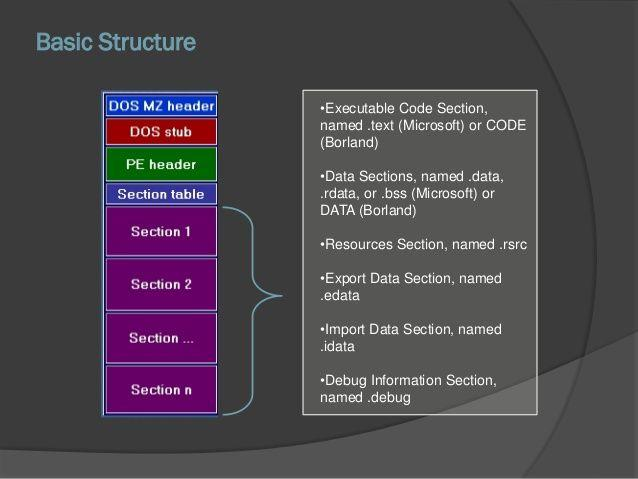
\includegraphics[width=\linewidth]{images/pe_header.jpg}
    \caption{Structure PE}
\end{figure}

    \subsubsection{En-tête MZ-DOS}
% pas sur de la phrase.
    Tout fichier PE doit commencer par l'en-tête MZ-DOS. Cet en-tête permet au système d'exploitation, au 
    moment de l'exécution d'un fichier, de reconnaître si c'est un exécutable valide ou non. \cite{pe2}

    \subsubsection{En-tête PE}
    Cet en-tête contient des champs d'information comme l'offset et la taille des zones de code et de données, 
    le système d'exploitation dont le fichier est destiné, la taille de la pile initial et 
    d'autre informations vitale. \cite{pe3}

    Les premiers bytes sont pris par MS-DOS stub qui a le rôle d'afficher un message d'erreur en cas ou 
    l'exécutable est lancé dans un environnement qui ne supporte pas Win32, les bytes suivant constitue 
    une structure de données appeler \emph{\textsc{image\_nt\_headers}} dont les champs sont :
    \begin{description}
        \item[image\_file\_header :] C'est une structure contenant les informations nécessaires
            sur le fichier comme le nombre de sections, le processeur dont le fichier est destiné \ldots etc.
        \item[image\_optional\_header :] C'est une structure contenant les des informations crucial comme l'adresse
            du point d'entrer.
    \end{description}

    \subsubsection{Les sections}
    Tous code, données et ressources sont stockés dans les sections. Une section se compose de deux 
    parties : une partie en-tête et une autre pour les données. Chaque en-tête est d'une longueur de 40 
    bytes ; il contient le nom de la section, la taille des données, l'offset de la section dans 
    le ficher PE, et l'adresse de début de la plage d'adresse du processus courant où la section doit être 
    chargé. \cite{pe4}

\section{Techniques de contournement des Anti-Virus}
    \subsection{Methodes de bases}
        \subsubsection{Methode cryptage/decryptage} Cette methode est faite en cryptant le corp du virus au préalable, puis le décrypter avec une boucle a son execution, elle permet d'éviter l'analyse statique.

        \subsubsection{Injection de code} Cette methode consiste ajouter un code externe au code d'un processus legale, ce qui fait qu'a l'execution, le code malveillant sera furtive et aura les memes prévileges que le code original.

        \subsubsection{Hallowing} Cette méthode consiste a suspendre un processus en éxécution puis de remplacer son code en memoire central par le code malveillant.

    \subsection{Méthodes alternatives}
        \subsubsection{L'offre a refuser} La principale limite avec les scanneurs des anti-virus est la quantité de temps qu'ils peuvent consacrer à chaque fichier . Lors d'une analyse régulière du système , l'anti virus devra analyser des milliers de fichiers alors il ne peut tout simplement pas passer trop de temps ou de puissance sur un fichier particulier ( ceçi pourrait également conduire à une forme de déni de service sur le l'AV ). On a comme exemple :
        \begin{itemize}
            \item Allocation d'une grande taille d'espace mémoire.
            \item Grand boucle a incrementation.
        \end{itemize}

        \subsubsection{Je ne pourrais pas faire cella} Cette technique ce base sur l'auto consience ce qui veux dire, est ce que le code est lancer dans l'environement de l'anti virus ou non.
            Cet environement ne donne pas accées a internet au virus qui est entrain d'etre scanner, alors si ce dernier essaye de telecharger ou d'accéder a une page web, l'environmenet générera une réponse que ce soit un fichier ou une page web,
            donc si le virus essaye d'accéder a une page web inexistante cella sera possible, ce qui n'est pas le cas dans un environement normal.

        \subsubsection{Connaitre l'ennemie} Si le nom d'utilisateur d'une machine est connu, il est possible de demander une action depedante de ce nom là, comme par exemple ecrire et lire dans les fichiers du compte utilisateur, donc si apres création d'un fichier et lecture de ce dernier ce conclu par un succeer cela veux dire que le virus n'est pas dans l'environement de l'AV.

        \subsubsection{Verifier l'enivronement}
        \begin{description}
            \item[Vérifier le nom de l'éxécutable :] Puisque le code est émulé, il ne démarre pas dans un processus qui a le nom du fichier binaire. Il suffit juste de vérifier si le premier argument contient le nom du fichier.

            \item[Vérifier la commande sleep :] Nous savons que les anti virus passe les intructions sleep, donc il suffit de verifier si la commande sleep a était bien exécuter ou non.
        \end{description}


% \section{Techniques de contournement des Anti-Virus}
%     \subsection{Methodes de bases}
%     \begin{description}
%         \item[Methode cryptage/decryptage :] Cette methode est faite en cryptant le corp du virus au préalable, puis le décrypter avec une boucle a son execution, elle permet d'éviter l'analyse statique.

%         \item[Injection de code :] Cette methode consiste ajouter un code externe au code d'un processus legale, ce qui fait qu'a l'execution, le code malveillant sera furtive et aura les memes prévileges que le code original.

%         \item[Hallowing :] Cette méthode consiste a suspendre un processus en éxécution puis de remplacer son code en memoire central par le code malveillant.
%     \end{description}

%     \subsection{Méthodes alternatives}
%     \begin{description}
%         \item[L'offre a refuser :] La principale limite avec les scanneurs des anti-virus est la quantité de temps qu'ils peuvent consacrer à chaque fichier . Lors d'une analyse régulière du système , l'anti virus devra analyser des milliers de fichiers alors il ne peut tout simplement pas passer trop de temps ou de puissance sur un fichier particulier ( ceçi pourrait également conduire à une forme de déni de service sur le l'AV ). On a comme exemple :
%         \begin{itemize}
%             \item Allocation d'une grande taille d'espace mémoire.
%             \item Grand boucle a incrementation.
%         \end{itemize}

%         \item[Je ne pourrais pas faire cella :] Cette technique ce base sur l'auto consience ce qui veux dire, est ce que le code est lancer dans l'environement de l'anti virus ou non.
%             Cet environement ne donne pas accées a internet au virus qui est entrain d'etre scanner, alors si ce dernier essaye de telecharger ou d'accéder a une page web, l'environmenet générera une réponse que ce soit un fichier ou une page web,
%             donc si le virus essaye d'accéder a une page web inexistante cella sera possible, ce qui n'est pas le cas dans un environement normal.

%         \item[Connaitre l'ennemie :] Si le nom d'utilisateur d'une machine est connu, il est possible de demander une action depedante de ce nom là, comme par exemple ecrire et lire dans les fichiers du compte utilisateur, donc si apres création d'un fichier et lecture de ce dernier ce conclu par un succeer cela veux dire que le virus n'est pas dans l'environement de l'AV.

%         \item[Verifier l'enivronement :]
%         \begin{description}
%             \item[Vérifier le nom de l'éxécutable :] Puisque le code est émulé, il ne démarre pas dans un processus qui a le nom du fichier binaire. Il suffit juste de vérifier si le premier argument contient le nom du fichier.

%             \item[Vérifier la commande sleep :] Nous savons que les anti virus passe les intructions sleep, donc il suffit de verifier si la commande sleep a était bien exécuter ou non.
%         \end{description}
%     \end{description}
% \section{Introduction}
% \section{Classification des virus par cible}
% \section{Classification des virus par techniques de dissimulations}
% \section{Les techniques d'infections}
% \section{Techniques de contournement des Anti-Virus}

\section{Conclusion}
À la fin de ce chapitre, des notions plus ou moins poussées concernant les virus --- comme les méthodes d'infections 
et les méthodes de dissimulation --- ont été abordés et étudiés. Ces notions sont indispensable pour cerner le 
mode de fonctionnement des virus, ainsi que pour la mise en œuvre du projet et du prochain chapitre.